\section{Patron de reconfiguration}

%
\begin{frame}{Comparaison des critères de réutilisation des décisions de reconfiguration
pour les SdSs}
\begin{onlyenv}<1->
\begin{table}[]
\renewcommand{\arraystretch}{2}
\resizebox{\textwidth}{!}{%
\centering
\begin{tabular}{|c|c|c|c|c|c|c|}
\hline
\backslashbox{Auteurs}{Critères}               & Titre     & Intention & Contexte  & Problème  & Solution  & Conséquence \\
\hline
Allen, 1998    & \ding{53} & \ding{53} & Partielle & Partielle & Partielle & \ding{53}   \\
\hline
Oliveira, 2015 & Partielle & \ding{53} & Partielle & Partielle & Partielle & \ding{53}   \\
\hline
Gomaa, 2004    & Partielle & \ding{53} & Partielle & \ding{53} &\ding{51}  & \ding{53}   \\
\hline
\end{tabular}
}
\end{table}
\end{onlyenv}
\begin{onlyenv}<2>
\begin{block}{}
\begin{itemize}
    \item Aider l'architecte à prendre en compte l'hétérogénéité et l'évolution du contexte de reconfiguration.
\end{itemize}
\end{block}
\end{onlyenv}
\end{frame}

%\begin{frame}{Réutilisation des décisions de %reconfiguration}
%\begin{columns}
%\begin{column}{0.5\textwidth}
%\textbf{Titre}\\
%Métaphore\\
%%\setlength\itemsep{0.7cm}
%\vspace{1mm}
%\textbf{Intention}\\
%Desc. informelle\\
%\vspace{1mm}
%\textbf{Contexte}\\
%Diagr. de block archi.
%\begin{itemize}
%\item utile à la compréhension d'un problème de %reconfiguration
%\item adapté à la modélisation de système complexe
%\end{itemize}                                                                   
%\textbf{Problème}\\
%Diagr. de block archi. source et ciblée 
%\begin{itemize}
%\item description des parties impliquées par la %reconf. 
%\end{itemize}
%\end{column}
%\begin{column}{0.5\textwidth}
%Desc. informelle invariants
%\begin{itemize}
%\item difficultés à résoudre
%\end{itemize}             
%Desc. informelle forces                                                         
%\begin{itemize}
%\item principe de la solution
%\end{itemize}             
%\textbf{Solution}\\
%Diagr. état + descript. informelle                                                              
%\begin{itemize}
%\item états du médiateur de reconf.
%\item opérations à implémenter
%\item événements de reconf.
%\end{itemize}             
%\textbf{Conséquence}\\
%Descr. informelle
%\begin{itemize}
%\item discutions des impactes sur les aspects non %fonctionnels
%\end{itemize}             
%\end{column}
%\end{columns}
%\end{frame}


\begin{frame}{Réutilisation des décisions de reconfiguration}
\textbf{Titre}\\
Métaphore\\
%\setlength\itemsep{0.7cm}
\vspace{5mm}
\textbf{Intention}\\
Description informelle\\
\vspace{5mm}
\textbf{Contexte}\\
Diagramme de block architecture
\begin{itemize}
\item utile à la compréhension d'un problème de reconfiguration
\item adapté à la modélisation de système complexe
\end{itemize}                                                                   
\end{frame}

\begin{frame}{Réutilisation des décisions de reconfiguration}
\textbf{Problème}\\
Diagramme de block architecture source et ciblée 
\begin{itemize}
\item description des parties impliquées par la reconfiguration 
\end{itemize}
Description informelle invariants
\begin{itemize}
\item difficultés à résoudre
\end{itemize}             
Description informelle forces      
\begin{itemize}
    \item principes de la solution
\end{itemize}

\end{frame}

\begin{frame}{Réutilisation des décisions de reconfiguration}
            
\textbf{Solution}\\
Diagr. état + descript. informelle                                                              
\begin{itemize}
\item états du médiateur de reconf.
\item opérations à implémenter
\item événements de reconf.
\end{itemize}   
\vspace{5mm}
\textbf{Conséquence}\\
Descr. informelle
\begin{itemize}
\item discutions des impactes sur les aspects non fonctionnels
\end{itemize}             

\end{frame}


\begin{frame}{Patron de reconfiguration co-evolution : intention}
\begin{columns}
\begin{column}{0.6\textwidth}
\begin{figure}
\centering
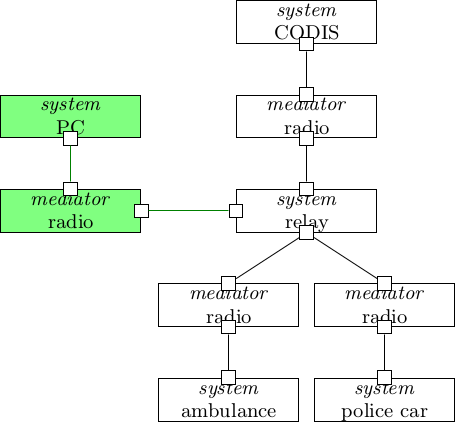
\includegraphics[height=5cm]{imgs/fig_rearchitecture}
\caption{\underline{\textbf{Exemple service des secours}}}
\end{figure}
\end{column}
\begin{column}{0.4\textwidth}
\underline{\textbf{Solution naïve} :}
\begin{itemize}
    \item application des changements implique une forte dégradation de service
\end{itemize}
\vspace{5mm}
\underline{\textbf{Solution proposée} :}
\begin{itemize}
    \item faire co-exister les CSs
\end{itemize}
\end{column}
\end{columns}
\end{frame}

\begin{frame}{Patron de reconfiguration co-evolution : délimitation du problème}
\begin{figure}
\begin{subfigure}[b]{0.45\textwidth}
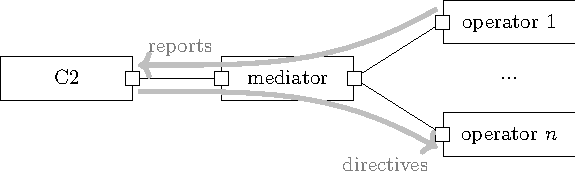
\includegraphics[width=5cm]{imgs/dc-context}
\caption{Contexte}
\end{subfigure}
\begin{subfigure}[b]{0.45\textwidth}
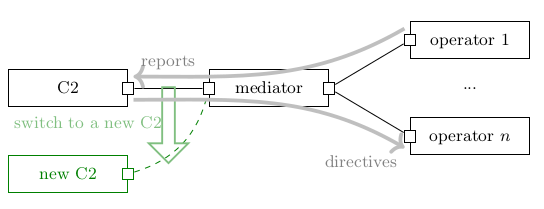
\includegraphics[width=5cm]{imgs/dc_archi-C2}
\caption{Problématique}
\end{subfigure}
\end{figure}

Invariants :
\begin{itemize}
\item Les deux C2 partagent la même connaissance de mission.
\item Tous les opérateurs sont connectés à exactement un
C2. 
\end{itemize}

Forces :
\begin{itemize}
\item Instancier une deuxième version du C2 qui coexiste avec
la version initiale.
\item Synchroniser les connaissances partagées entre les versions du
C2.
\end{itemize}

\end{frame}

\begin{frame}{Patron de reconfiguration co-evolution : description de la solution}
\begin{figure}
\centering
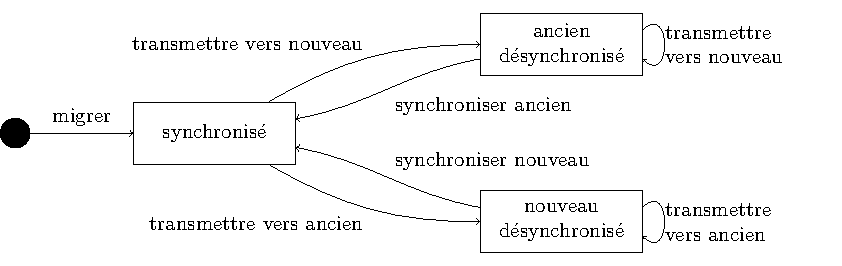
\includegraphics[width=10cm]{imgs/slide_solution_coevolution.pdf}
\end{figure}
%\begin{tiny}
Conséquences :
\begin{itemize}
\item Les C2 ont toujours connaissance de l’historique des communications des CSs opérationnels.
\item La disponibilité des services du C2 est maintenue pendant la reconfiguration.
\item Les performances du SdS affectées pendant la reconfiguration si opérations de synchronisation réalisées. Baisse de performance peut être compensée par mécanismes de transactions concurrentes
\end{itemize}
%\end{tiny}
\end{frame}


\begin{frame}{Patrons de reconfiguration supplémentaires}
\begin{itemize}
\setlength\itemsep{0.7cm}
\item \underline{\textbf{Quiescence}} : rendre passifs
les composants dépendant du composant ciblé par la reconfiguration. 
\item \underline{\textbf{Tranquilité}} : variante de la quiescence qui assouplit
les critères de reconfiguration. Elle décrit les conditions dans
lesquelles la reconfiguration peut être réalisée sans attendre l'état de
quiescence.
\item \underline{\textbf{Co-evolution}} : déployer directement la nouvelle version du composant ciblé par la
reconfiguration. Les deux versions d'un
composant s'exécutent simultanément. 
\item \underline{\textbf{Opportuniste}} : une opération de
déconnexion et connexion qui est réalisée dès que l'occasion se
présente.  
\end{itemize}
\end{frame}
